\subsection{Verification}
The exact transient solution for a supercapacitor under galvanostatic charge
conditions is given in \cite{Subramanian2004}.  The model includes both
double-layer charging and faradaic prossesses approximated with linear
kinetics.

The overpotential and interfacial current density expressed dimensionless
form, $\eta^*$ and $i_n^*$ respectively, are
functions of the dimensionless current density $\delta$,
dimensionless exchange current density $\nu^2$,
and the ratio of the solution phase to matrix phase conductivities $\beta$.
\begin{align}
    \delta = I \frac{F L}{\kappa R T} , \quad
    \nu^2 = \frac{ai_0 (\alpha_a+\alpha_c) F L^2}{R T} \left( \frac{1}{\sigma} + \frac{1}{\kappa} \right) , \quad
    \beta = \frac{\kappa}{\sigma} \nonumber
\end{align}

\begin{align}
    \eta^* =
    \frac{\delta (1 + \beta) \exp(-\nu^2 \tau)}{\nu^2}
    - \frac{\delta \left( \cosh(\nu [1-X]) + \beta \cosh(\nu X) \right)}{\nu \sinh(\nu)} \nonumber \\
    + 2\delta \sum_{n=1}^{\infty} \frac{\beta \cos(n \pi) + 1}{\nu^2 + n^2 \pi^2} \cos(n \pi X) \exp(-(n^2 \pi^2 + \nu^2) \tau)
\end{align}

\begin{align}
    i_n^* =
    - 2\delta \sum_{n=1}^{\infty} \frac{\beta \cos(n \pi) + 1}{(\nu^2 + n^2
\pi^2) (\beta + 1)} n^2 \pi^2 \cos(n \pi X) \exp(-(n^2 \pi^2 + \nu^2) \tau) \nonumber \\
    - \frac{\delta \nu \left( \cosh(\nu [1-X]) + \beta \cosh(\nu X) \right)}{(\beta + 1) \sinh(\nu)}
\end{align}
with
\begin{equation}
    X = \frac{x}{L} , \quad
    \tau = \frac{t}{aC (1/\kappa + 1/\sigma) L^2} , \quad
    \eta^* = \frac{\eta F}{R T} .
\end{equation}

The potential drop across the porous electrode is computed as
\begin{equation}
    V^* =
    \frac{\eta^*|_{X=0} + \beta \eta^*|_{X=1} - \delta \beta}{1 + \beta}
\end{equation}

The total voltage (two porous electrode with a separator between them) can be
evaluated using
\begin{equation}
    U = 2 \frac{R T}{F} V^* + I \frac{L_s}{\kappa}
    \label{eq:voltage_drop_across_two_electrodes_and_separator}
\end{equation}
where $L_s$ is the thickness of the separator.  Electrical resistivity in the
current collectors is very low.  Their contribution to the total voltage is
not accounted for in the exact solution.  It is assumed that there is little
or no effect on the verification procedure.

The following input is used for the energy storage device.
{\tiny
\begin{lstlisting}
<geometry>
    <electrode_width>50.0e-6</electrode_width> <!-- metre -->
    <separator_width>25.0e-6</separator_width> <!-- metre -->
    <collector_width>5.0e-6</collector_width> <!-- metre -->
    <sandwich_height>25.0e-6</sandwich_height> <!-- metre -->
    <tab_height>5.0e-6</tab_height> <!-- metre -->
</geometry>
<material_properties>
    <differential_capacitance>0.03134</differential_capacitance> <!-- farad per square metre -->
    <separator_void_volume_fraction>0.6</separator_void_volume_fraction>
    <electrode_void_volume_fraction>0.67</electrode_void_volume_fraction>
    <electrolyte_conductivity>0.067</electrolyte_conductivity> <!-- siemens per metre -->
    <solid_phase_conductivity>52.1</solid_phase_conductivity> <!-- siemens per metre -->
    <collector_electrical_resistivity>28.2e-9</collector_electrical_resistivity> <!-- ohm metre -->
    <bruggemans_coefficient>1.5</bruggemans_coefficient>
    <electrode_tortuosity_factor>2.3</electrode_tortuosity_factor>
    <separator_tortuosity_factor>1.29</separator_tortuosity_factor>
    <pores_characteristic_dimension>1.5e-9</pores_characteristic_dimension> <!-- metre -->
    <pores_geometry_factor>2.0</pores_geometry_factor>
    <exchange_current_density>0.7463e-5</exchange_current_density> <!-- ampere per square metre -->
</material_properties>
\end{lstlisting}
}
The supercapacitor, initially fully discharged, undergoes constant current
charge at $\unit{5}{\milli\ampere}$ which correspond to a total current
density $I=\unit{200}{\amperepersquaremetre}$ throughout the electrode.
This yields
$\delta = 19.8191$,
$\nu^2 = 0.0495684$, and
$\beta = 0.000374614$.
The voltage $U$ at time $t=\unit{0.1}{\second}$ is computed as the grid
resolution is increased.

The discretization error is calculated using the exact transient solution
given above in Eq.~\eqref{eq:voltage_drop_across_two_electrodes_and_separator}.
\begin{equation}
    \mathrm{error\ \%} =
    \left| \frac{U_{computed} - U_{exact}}{U_{exact}} \right| \times 100
\end{equation}
In order to ensure that temporal discretization error does not interfere in
the spatial convergence study, the time step $\Delta t$ is refined until a
plateau is reached, as can be seen on Fig.~\ref{fig:error_convergence} on the
left.  The spatial error is then plotted against the number of grid cells in
Fig.~\ref{fig:error_convergence} (right).  The results correspond to a
two-dimensional problem ($d=2$) using piecewise-linear basis functions
$\varphi_i$ (degree $p=1$).  The slope on the log-log graph is -1 which is the
expected behavior $-(p+1)/d$.
\begin{figure}
    \begin{subfigure}{0.49\textwidth}
        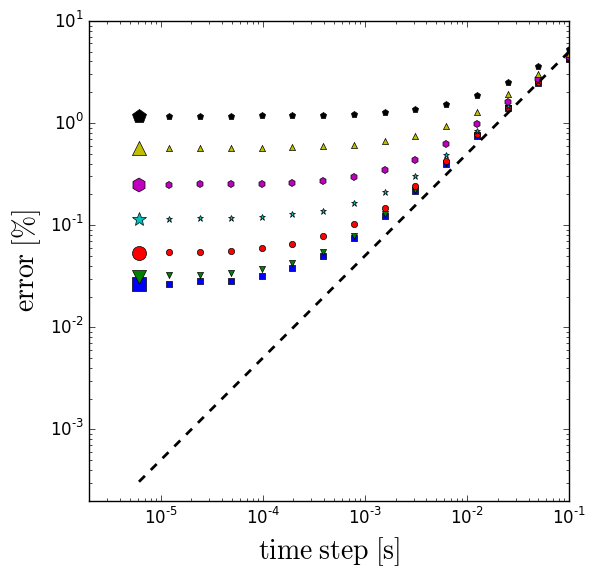
\includegraphics[width=\textwidth]{figures/temporal_error_convergence}
    \end{subfigure}
    \begin{subfigure}{0.49\textwidth}
        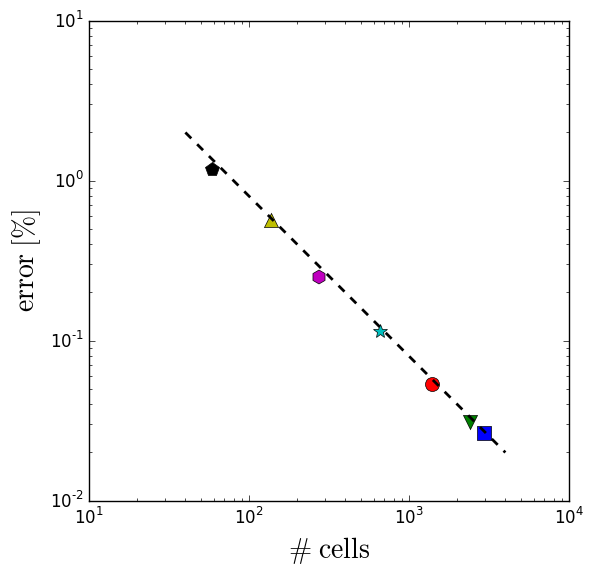
\includegraphics[width=\textwidth]{figures/spatial_error_convergence}
    \end{subfigure}
    \caption{Discretization error in the total voltage with piecewise-linear
    basis function in 2-D.
    Left:  Eliminating the temporal discretization errors.
    Right:  Convergence of the spatial  error.}
    \label{fig:error_convergence}
\end{figure}

